\section{Эксперименты}

\subsection{Предлагаемые улучшения}


Модель BBS-Net представленная в \cite{BBS} была взята в качестве бейзлайна. При её тренировке в качестве функции
ошибки использовалась  бинарная перекрёстная энтропия, а бекбоном выступала свёрточная сеть ResNet-50\cite{ResNet}
с претренированными весами из библиотеки torchvision \footnote{\url{https://pytorch.org/vision/stable/models.html}}.

Цель наших эксперимента - улучшить метрики качества исходного бейзлайна путём использования 
других функций потерь, а также изменением исходного бекбона с ResNet-50 на EfficientNet b-0\cite{Efficientnet}.
Согласно \cite{Efficientnet}, в сравнении с ResNet-50 сеть EfficientNet b-0 имеет большую точность 
и в 4.9 раз меньше параметров (5.3M против 26M). Таким образом, в ходе экспериментов мы надеемся 
не только улучшить качество метрик, но и уменьшить размер модели, а также ускорить её работу.


\subsection{Функции потерь}


// TODO мб про лоссы и метркии сразу писать с точки зрения задачи СОД с обозначениями S и G?

Для тренировки нейронных сетей используют различные алгоритмы, основанные на стохастическом градиентном спуске,
для максимизации или минимизации некоторой целевой функции. В качестве целевой функции используют различные функции потерь, 
которые нужно минимизировать. Вид этих функций зависит от типа решаемой задачи, а выбор подходящей функции напрямую влияет на 
качество обучаемой модели. 

Для решения задачи выявления самых заметных объектов на изображении 
во многих работах, в том числе и в исследуемой нами \cite{BBS}, применяется функция бинарной перекрёстной энтропии.

В результате работы модели мы ожидаем получить бинарной изображение, которое содержит выделение наиболее заметных областей. 
Другими словами, мы хотим классифицировать каждый пиксель на изображении и отнести его либо к группе "выделяющихся", либо "не выделяющихся". То есть,
решить задачу сегментации - классификации пикселей на изображении. Таким образом, использование бинарной перекрестной энтропии 
в качестве функции потерь вполне естественно.

Однако, за последние годы для улучшения результатов задачи сегментации изображений были предложены и другие функции потерь, подходящие для 
этой задачи \cite{Loss-Functions}. Среди них : 


// TODO: русифицировать заголовочки

\begin{itemize}
    \item Dice Loss \cite{Dice-Loss}
    \item Jaccard Loss(Intersection over Union) \cite{IoU-Loss}
    \item Focal Loss \cite{Focal-Loss}
\end{itemize}

Остановимся подробнее на каждой из приведённых функций.

// TODO ввести обозначения y и ypred
// TODO поменять $\hat{y} $ на $\hat{p}$

\subsubsection{Бинарная Перекрёстная Энтропия}

Функция бинарной перекрёстной энтропии(binary cross entropy) является частным случаем функции перекрёстной энтропии - одной из самых популярных 
функций потерь для задач классификации и, как следствие, сегментации - попиксельной классификации.

Перекрёстная энтропия \cite{CE} определяется следующим образом: 
\begin{equation}
    L_{CE} = -\sum_{i=1}^{C}y_c\log{\hat{y_c}}
\end{equation}
где $y$ - истинный класс объекта, $y_c$ - предсказанный класс, а $C$ - количество 
всех классов.

В случае предсказания только двух классов, то есть при $C=2$, 
и возможных значениях меток $y \in \{0,1\}$
перекрёстная энтропия превращается в бинарную:

\begin{equation}
    L_{CE} = -\sum_{i=1}^{2}y_c\log{\hat{y_c}} = 
    -(y\log{\hat{y}} + (1-y)\log{1-\hat{y}})
\end{equation}

\subsubsection{Dice Loss} 

Коэффициент Дайса широко используется в компьютерном зрении для оценки сходства 
между двумя изображениями. В работе \cite{Dice} была предложена адаптация коэффициента 
для использования его в качестве функции потерь 

\begin{equation}
    L_{DL}(y, \hat{p} ) = 1 - \frac{2y\hat{p} + 1}{y + \hat{p} + 1}
\end{equation}

//TODO - единички поменять на параметр смуз? 

\subsubsection{IoU Loss}

Коэффициент Жаккара, использующийся как мера 
сходства и различия двух множеств \cite{IoU-Loss}:

\begin{equation}
    J(A,B) = \frac{|A \cap B|}{|A \cup B|} = \frac{|A \cap B|}{|A + B - A \cap B|}
\end{equation}

Это отношение также называют пересечением над объединением 
(Intersection over Union, IoU). В контексте задач сегментации и детекции, 
оно позволяет определить, насколько 
хорошо предсказанная моделью область изображения перекрывает
область искомую.

Коэффициент Жаккара легко может быть преобразован в функцию потерь\cite{IoU-Loss-2}:

\begin{equation}
    L_{IoU} = 1- \frac{|A \cap B|}{|A \cup B|} = 1 - \frac{|A \cap B|}{|A + B - A \cap B|}
\end{equation}

\subsubsection{Focal Loss}

//TODO edit

Фокальная функция потерь Лол, представленный в работе \cite{Focal-Loss}, является вариацией бинарной перекрёстной энтропии.
Отличительной чертой этой функции является возможность снижать вклад простых примеров и фокусироваться на примерах, более сложных
для обучения. //TODO чего?
В частности, функция хорошо показывает себя в случае сильно несбалансированных классов.
Например, в случае когда сегментированная область гораздо меньше изображения.

Как выводится фокал лосс из кросс энтропии //// ТУдУ

\begin{equation}
    CE=\begin{cases}
        -\log{p} & \text{if }y=1\\
        -\log{1-p} & \text{if }y=0
     \end{cases}
\end{equation}

Для удобства введём новое обозначение оценочной вероятности класса:

\begin{equation}
    p_t=\begin{cases}
        p & \text{if }y=1\\
        1-p & \text{if }y=0
     \end{cases}
\end{equation}

Тогда функцию перекрёстной энтропии можно переписать как

\begin{equation}
    CE(p,y) = CE(p_t) = -\log{p_t}
\end{equation}

Фокальная функция потерь имеет вид

\begin{equation}
    FL(p_t) = -\alpha_t(1-p_t)^{\gamma}\log{p_t}
\end{equation}
 

Focal Loss proposes to down-weight easy examples and focus
training on hard negatives using a modulating factor,

//TODO: тут он с помощью коэффициента навидываем не просто "сложным", 
а hard negatives . Как бы это описать 


\subsection{Метрики Качества}

//TODO  Сразу про пиксели и СОД! переделать обозначения

В качестве метрик качества мы будем использовать две наиболее широко используемых в задачах SOD метрики: 
среднюю абсолютную ошибку (Mean Absolute Error, MAE) и F-меру(F-measure).

Средняя абсолютная ошибка - это сумма разностей модулей соответствующих значений пикселей предсказанного и истинного изображения.// TODO?
\begin{equation}
    mae = \frac{1}{N}\sum_{i=1}^N|y_i - \hat{p_i}|
\end{equation}

F-мера //TODO

\begin{equation}
    F_1 = 2\frac{precision \times recall}{precision + recall}
\end{equation}
где $precision$ //TODO

\subsection{Данные для экспериментов}

С растущим интересом к задаче RGBD-SOD, а также с распространением устройств, способных 
снимать изображением с картой глубины, за последние несколько лет появилось несколько RGB-D SOD датасетов.

Каждый датасет состоит из изображения с соответствующей ему картой глубины, а также
бинарное изображение с маской искомого выделяющегося объекта на изображении.

//TODO побольше про девайсы расписать!

// TODO примерчик с картиночками

//TODO описание поподробней бы

// TODO таблчика как в https://arxiv.org/pdf/2008.00230.pdf или в https://arxiv.org/pdf/1907.06781.pdf

Ниже представлен краткий обзор существующих датасетов:
\begin{itemize}
    \item STERE \cite{STERE} - первый датасет со стереоскопическими изображениями, собранных с сайтов Flickr, NVIDIA 3D Vision Live и Stereoscopic Image Gallery
    Содержит 1000 изображений с различными разрешениями // TODO: добавить ссылки-сноски
    \item GIT \cite{GIT} - содержит 80 картинок домашней обстановки, собранных роботом.
    \item LFSD \cite{LFSD}
    \item DES \cite{DES} - небольшой датасет объёмом 135 изображений, собранных с помошью Microsoft Kinect. Разрешение изображений: 640х480.
    \item NLPR \cite{NLPR} - содержит 1000 изображений разрешением 640х480, также собранных с помошью Microsoft Kinect.
    \item NJU2K \cite{NJU2K} - самый большой датасет, содержащий 1985 изображений с разными разрешениями, собранных из интернета, 3D фильмов и снятых на стерео камеру Fuji W3.
    \item SSD \cite{SSD} - содержит 80 картинок с высоким разрешением 960х1080, собранных из 3D фильмов.
    \item DUT-RGBD \cite{DUT} - содержит 1200 изображений со сложными для модели факторами, например: однотипный передний план или похожие передние и задние планы
    \item SIP \cite{Rethinking-RGBD} - содержит 1000 изображений с разрешением 992х744, снятых на смартфон
\end{itemize}

В таблице [ссылка на таблицу] представлены характеристики датасетов, год выхода, количество изображений и их разрешение.

\begin{center}
    \begin{table}
        \begin{tabular}{|c|c|c|c|c|} 
            \hline
            Датасет & Год & Размер & Разрешение\\
            \hline
            \hline
            STERE\cite{STERE} & 2012 & 1000 & $[251 \sim 1200] \times [222 \sim 900]$ \\
            \hline
            GIT\cite{GIT} & 2013 & 80 & $640 \times 480$ \\
            \hline
            LFSD\cite{LFSD} & 2014 & 100 & $360 \times 360$ \\
            \hline
            DES\cite{DES} & 2014 & 135 & $640 \times 480$  \\
            \hline
            NLPR\cite{NLPR} & 2014 & 1000 &  $640 \times 480$ \\
            \hline
            NJU2K\cite{NJU2K} & 2014 & 1985 & $[231 \sim 1213] \times [274 \sim 828]$\\
            \hline
            SSD\cite{SSD} & 2017 & 80 & $960 \times 1080$\\
            \hline
            SIP\cite{Rethinking-RGBD} & 2020 & 929 &  $992 \times 744$\\
            \hline
        \end{tabular}
    \caption{Эксперименты}
    \label{tab:datasets}
    \end{table}
\end{center}


Каждую модель мы будем обучать и валидировать на датасете NJU2K. Остальные датасеты будут тестовыми. На них мы будем
запускать обученные модели и считать метрики качества.

\subsection{Описание эксперимента}

% ----
Имплементация моделей, код для тренировки и валидации, функций потерь и метрик качества были написаны на языке Python 3.8
с использованием фреймворка для глубокого обучения Pytorch 1.8.0\cite{Pytorch}.

% про ббс 
В работе была использована оригинальная имплементация модели от авторов статьи \cite{BBS}, которая доступна на GitHub [ссылка!].
На её основе была написана модель BBS-Net, которая в качестве свёрточной сети для извлечения признаков
использовала сеть EfficientNet-B0 \cite{Efficientnet} с весами, предобученными на датасете ImageNet.\footnote{\url{https://github.com/lukemelas/EfficientNet-PyTorch}} 


Все модели тренировались и валидировались на датасете NJU2K предварительно разделённым на NJU2K\_TRAIN для тренировки, 
который содержит 1485 изображений, и NJU2K\_TRAIN для промежуточной валидации, содержащий 500 изображений.
Каждая тренировка состояла из 150 эпох с размером пакета(batch size) равным 10. В конце каждой эпохи запускалась валидация: рассчитывалось среднее
значение функции потерь и средней абсолютной ошибки(MAE), минимальное значение которой сохраняется и обновляется во время
всего процесса тренировки. В случае обновления значения - текущее состояние модели сохраняется и помечается наилучшим в смысле качества обучения.
В результате тренировки мы получаем модель, которая показывает наименьшую ошибку на валидационном датасете. Такая стратегия используется для того,
чтобы избежать переобучения под тренировочный датасет. 
Для тренировки модели использовался стандартный оптимизатор Adam\cite{Adam}. Начальное значение параметра скорости обучения(learning rate) 
равно 0.0001. Каждые 60 эпох значение уменьшалось в 10 раз \ref{fig:lr}. Такой подход был предложен в оригинальной работе \cite{BBS}.


\begin{figure}[h]
    \centering
    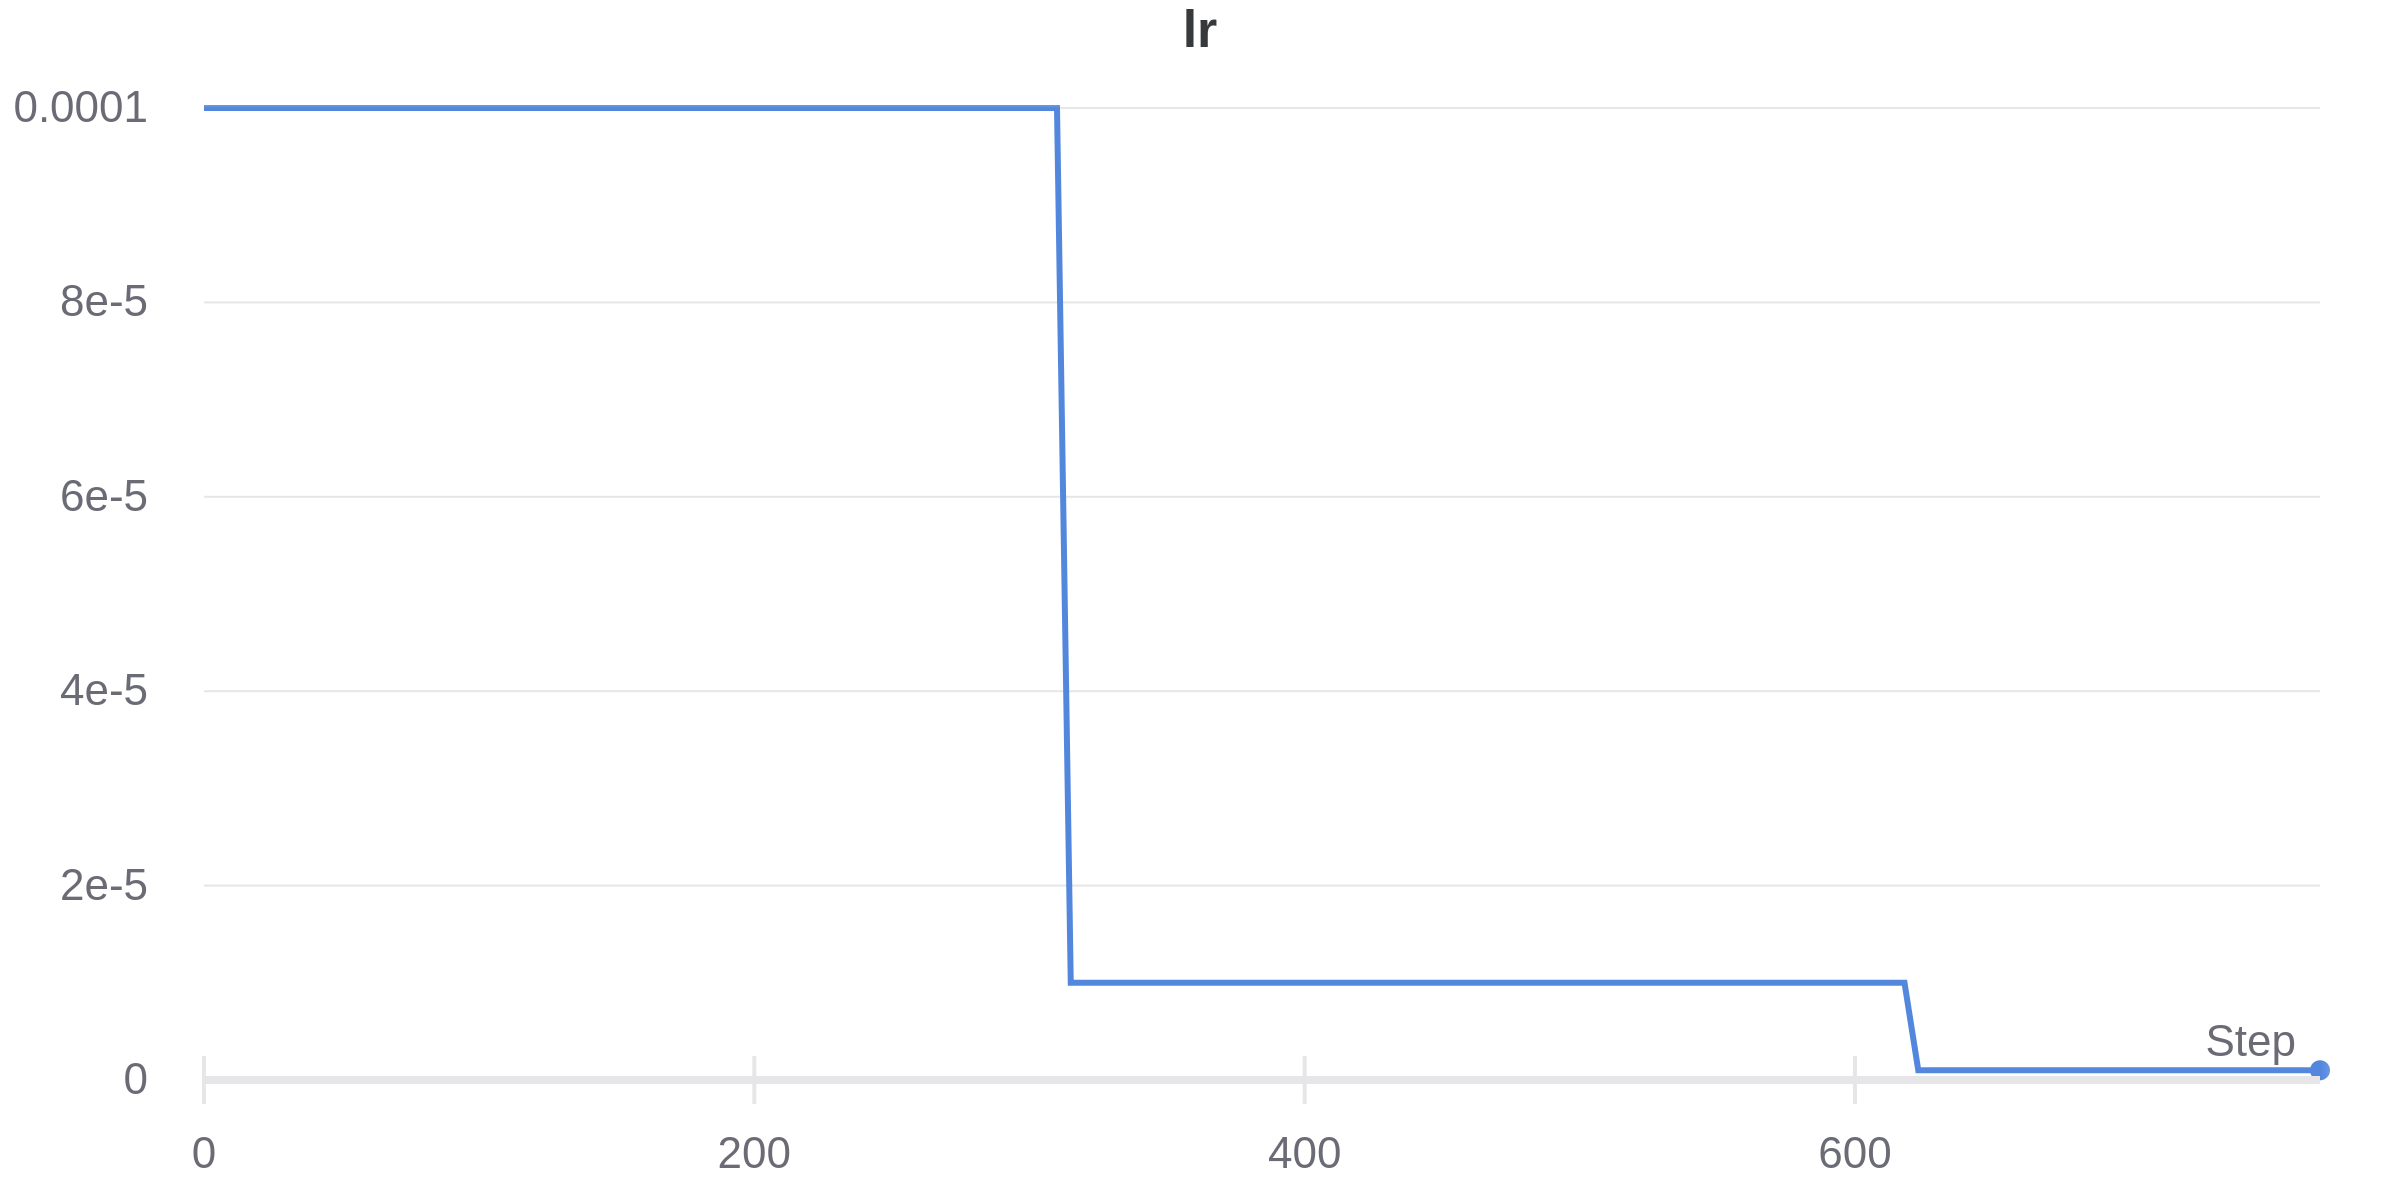
\includegraphics[width=1\textwidth]{lr}
    \caption{Изменения скорости обучения при тренировке}
    \label{fig:lr}
\end{figure}

На вход модели подаются RGB изображение и карта глубины с разрешением 352х352 как на этапе тренировки, там и на этапе расчёта тестовых метрик.
Так как изображения в датасетах имеют разные размеры, перед передачей применяется изменение размера, а также, на этапе тренировки, некоторые приёмы аугментации 
изображения: поворот, масштабирование, кроп. Все преобразования выполняются через стандартные классы для работы с данными в Pytorch: Dataset и DataLoader
\footnote{\url{https://pytorch.org/docs/stable/data.html}}
Все эксперименты проводились на платформе Google Colab\footnote{\url{https://colab.research.google.com/notebooks/intro.ipynb}}
с GPU Tesla P100-PCIE-16GB.



%Таблчика с экспериментами

\begin{center}
    \begin{table}
        \begin{tabular}{ |c c|c|c|c|c|c|c|c|c| } 
            \hline
            \multirow{2}{*}{\rotatebox[origin=c]{90}{Датасет}} & \multirow{2}{*}{Метрика} & \multicolumn{4}{ |c| }{ResNet} & \multicolumn{4}{ |c| }{EfficientNet} \\
            \cline{3-10}
            & & BCE & focal & dice & IoU & BCE & focal & dice & IoU\\
            \hline
            \multirow{2}{*}{\rotatebox[origin=c]{90}{NJU2K}} & mae $\downarrow$ &0,033&0,06&0,031&0,032&0,035&0.057&0,031&\textbf{0,030} \\
            & f1  $\uparrow$ &0,909&0,832&\textbf{0,920}&0,915&0,901&0.842&0,916&0,918\\
            \multirow{2}{*}{\rotatebox[origin=c]{90}{NLPR}} & mae $\downarrow$ &0,041&0,065&0,040&0,037&0,040&0.059&0,039&\textbf{0,034} \\
            & f1  $\uparrow$ &0,840&0,734&0,856&0,858&0,838&0.756&0,846&\textbf{0,865}\\
            \multirow{2}{*}{\rotatebox[origin=c]{90}{DES}} & mae $\downarrow$ &0,019&0,041&0,017&\textbf{0,015}&0,019&0.039&0,016&0,016\\
            & f1  $\uparrow$ &0,916&0,819&0,930&\textbf{0,939}&0,918&0.822&0,933&0,929\\
            \multirow{2}{*}{\rotatebox[origin=c]{90}{SSD}} & mae $\downarrow$ &0,046&0,073&0,044&0,046&0,047&0.068&0,043&\textbf{0,041} \\
            & f1  $\uparrow$ &0,841&0.777&0,855&0,851&0,844&0.777&0,860&\textbf{0,863}\\
            \multirow{2}{*}{\rotatebox[origin=c]{90}{STERE}} & mae $\downarrow$ &0,039&0,066&0,037&\textbf{0,035}&0,039&0.063&0,037&0,036 \\
            & f1  $\uparrow$ &0,888&0,817&0,898&\textbf{0,905}&0,891&0.824&0,899&0,903\\   
            \multirow{2}{*}{\rotatebox[origin=c]{90}{LFSD}} & mae $\downarrow$ &0,077&0,104&\textbf{0,066}&0,072&0,074&0.102&0,082&0,072\\
            & f1  $\uparrow$ &0,843&0,782&\textbf{0,862}&0,859&0,843&0.789&0,834&0,851\\  
            \multirow{2}{*}{\rotatebox[origin=c]{90}{SIP}} & mae $\downarrow$ &0,047&0,07&0,045&0,044&0,047&0.069&0,051&\textbf{0,042}\\
            & f1  $\uparrow$ &0,867&0,789&0,877&0,88&0,87&0.809&0,859&\textbf{0,884}\\  
            \multirow{2}{*}{\rotatebox[origin=c]{90}{DUT}} & mae $\downarrow$ &0,121&0,145&0,116&0,121&0,112&0.122&\textbf{0,105}&0,14\\
            & f1  $\uparrow$ &0,592&0,574&0,67&0,597&0,65&0.639&0,707&\textbf{0,728}\\  
            \hline
        \end{tabular}
    \caption{Эксперименты}
    \label{tab:experiments}
    \end{table}
\end{center}


Первая колонка - бейзлайн //TODO расписать

Результаты эксперимента описаны в таблице \ref{tab:experiments}. 
Видно, что специализированные функции потерь для задачи сегментации
показали свою эффективность. Лучшие результаты метрик на всех исследованных
датасетах показали модели, обученные либо с dice loss, либо с IoU loss//TODO
При этом, модели, обученные с IoU loss лучшие по обеим метрикам
на датасетах NLPR, DES, SSD, STERE, SIP. Модели, обученные с Dice loss 
по обеим метрикам лучшие только на датасете LFSD.

Эксперимент с заменой свёрточной сети для извлечения признаков с ResNet на EfficientNet b-0 
так же оказался удачным. На половине датасетов модели на основе EfficientNet b-0 показали 
лучшие результаты по обеим метрикам и на датасете NJU2K - лучший результат по метрике $mae$.

При этом, новые модели опережают результаты бейзлайна.

//TODO картинки с по датасетам: бейзлайн/лучший? 

